\section{Results: Propagation and Blockage}
\label{sec:results-propagation}

\subsection{Mixed LOS and NLOS Propagation}
\label{subsec:mixed}

% src: mixed_propagation_2026_09/seed_repeats_all_models_summary.json (verdict: overall paired gains 11.4-15.4%, all significant; per-run multi/single maes for paired per-group gains; ranking h=5 16.98-17.34 for ranks 1-6); history_gain_by_zone_summary.json (h=0 test samples LOS 21,866 / NLOS 7,938)
Giving the four regions of the macro cell their own LOS or NLOS propagation leaves the main result intact~(Figure~\ref{fig:mixed-gain}). About three quarters of test samples now fall in LOS regions. History lowered the overall error of all seven models, by $11$ to $15\%$, with every seed-paired confidence interval clear of zero. For multi-antenna devices the gains are $2.3$ to $3.9\,\text{m}$, as on the uniform-NLOS data, and the six trained models other than $k$-NN again lie within $0.4\,\text{m}$ of each other. The single-antenna result differs: both tree ensembles now gain about $1.6\,\text{m}$ for single-antenna devices, while the neural models and $k$-NN do not.

\begin{figure}[h]
  \centering
  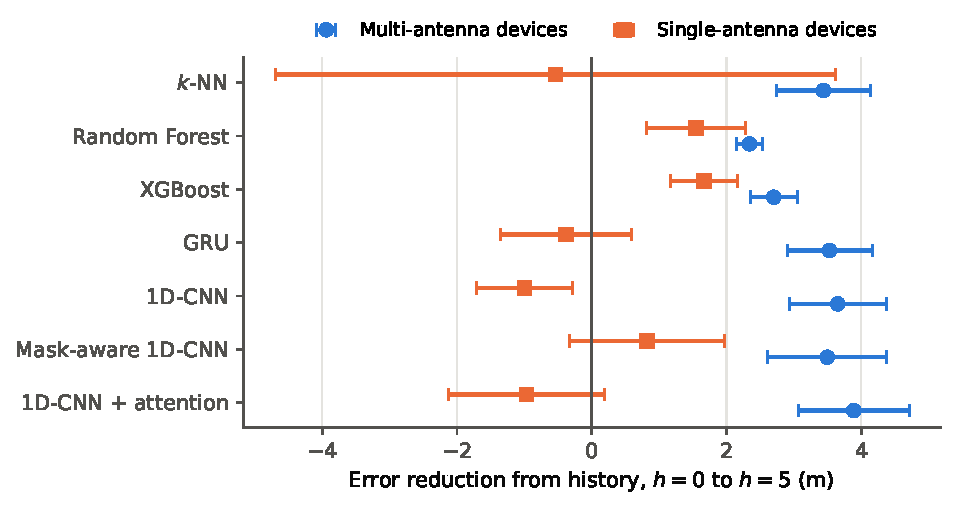
\includegraphics[width=0.8\textwidth]{fig_mixed_history_gain_ci}
  \caption{Reduction in mean error from adding history~($h=0$ to $h=5$), per model and device group, mixed-propagation realization of the macro-cell study. Seed-paired means over five user splits with $95\%$ confidence intervals.}
  \label{fig:mixed-gain}
\end{figure}
% src: figure_scripts/make_figures_diagnostic.py mixed_history_gain_ci()

% src: mixed_propagation_2026_09/pathloss_fit_summary.json zones.LOS (gamma 2.578, sigma 7.67 dB, R^2 0.261) and zones.NLOS (gamma 3.595, sigma 11.89 dB, R^2 0.069); per-region fits are unstable (e.g. residential gamma 6.92) and are not used; note: the fit assigns regions geometrically from the Voronoi centres
Signal strength is more informative about range in the LOS regions. A path-loss fit to the LOS samples gives $\gamma = 2.58$ with a shadowing spread of $7.7\,\text{dB}$, and range explains $26\%$ of the variance in RSS. In the NLOS regions the fit gives $\gamma = 3.60$, a spread of $11.9\,\text{dB}$, and only $7\%$ of the variance explained.

% src: mixed_propagation_2026_09/history_gain_by_zone_summary.json verdict (LOS 15.94%, NLOS 8.65%; mean range LOS 90.1 m, NLOS 96.8 m; XGBoost, seed 42); diagnostics_2026_10/mixed_propagation summary.<model>.<cond>.multi.gain_vs_snap_by_los (XGB angle LOS 3.12+-0.62, NLOS 1.51+-0.16; RF angle 2.68+-0.33 / 1.25+-0.15; XGB rss 0.33+-0.22 / 0.38+-0.25)
History helps more in LOS regions, and the difference lies in the angle channels~(Figure~\ref{fig:los-nlos}). In a single XGBoost run, history lowered error by $15.9\%$ in LOS regions and by $8.7\%$ in NLOS regions. Mean range is slightly shorter in the LOS regions~($90$ against $97\,\text{m}$), but too little to account for the difference. Splitting the channel-group test by region shows where the difference comes from: for multi-antenna devices, angle history lowered XGBoost's error by $3.12 \pm 0.62\,\text{m}$ in LOS regions and by $1.51 \pm 0.16\,\text{m}$ in NLOS regions, and Random Forest shows the same ratio, while RSS history gave the same small gain in both. Under LOS a single dominant path makes the measured angle a steadier function of position, which is consistent with a sequence of angles carrying more about range there.

\begin{figure}[h]
  \centering
  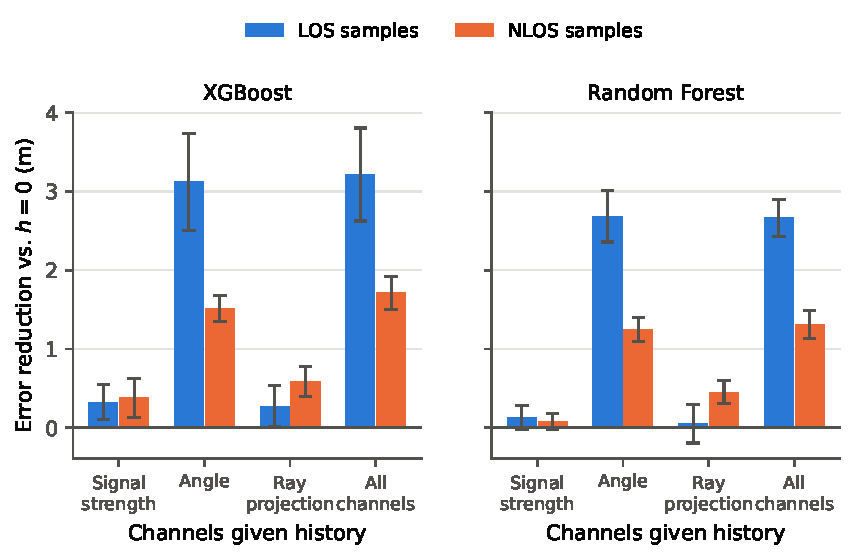
\includegraphics[width=0.85\textwidth]{fig_los_nlos_channels}
  \caption{Reduction in mean error against the $h=0$ input for multi-antenna devices, by channel group given history and by whether the current sample lies in a LOS or NLOS region, mixed-propagation realization. Seed-paired means over five user splits with $95\%$ confidence intervals.}
  \label{fig:los-nlos}
\end{figure}
% src: figure_scripts/make_figures_diagnostic.py los_nlos_channels()

% src: diagnostics_2026_10/mixed_propagation summary.xgboost.rss_hist.single.gain_vs_snap_by_los (LOS 1.28+-0.42, NLOS 1.53+-0.87); exploratory check on errors_first_seed.npz (seed 42, full vs snap, single-antenna samples whose six-step window contains both LOS and NLOS samples, 15% of single-antenna samples): RF 2.85 vs 1.06 m, kNN 2.92 vs 0.84 m, XGB 1.40 vs 1.16 m (scratch analysis analyze_b6_npz.py)
The single-antenna gain from RSS history on these data is not explained by the cleaner LOS path-loss relation: XGBoost's RSS-only gain is $1.28 \pm 0.42\,\text{m}$ for samples in LOS regions and $1.53 \pm 0.87\,\text{m}$ for samples in NLOS regions. A possible source is the step in signal strength that occurs when a device crosses from one propagation region to another, which marks a location the window can recognize. In one split, the gain for Random Forest and $k$-NN was about three times larger when the history window spanned such a crossing than when it did not~($2.9$ against $1.1\,\text{m}$ for Random Forest), but XGBoost showed no such difference, and windows without a crossing still gained about $1\,\text{m}$. This is a lead from a single split with ten single-antenna users, not an explanation, and the single-antenna gain on mixed-propagation data remains open.

\subsection{A Blocked Line of Sight}
\label{subsec:blocked}

% src: CONTINUE_HERE.md §4 (prediction: advantage grows with blockage duration until the pre-blockage heading stops being informative, then decays); blocked_los_2026_09/b6_seed*_summary.json (5 seeds, XGBoost, h in {0,5}): blocked gain 28.9/28.5/36.5/28.6/22.8% mean 29.1 sd 4.9; unblocked mean 22.5 sd 6.0; blocked h0 18.90 -> h5 13.45 m, unblocked 25.08 -> 19.59 m; paired blocked-minus-unblocked gain in metres -0.04 +- 0.46; by width 24.1/25.4/23.8/26.8/31.6/27.4/26.3/32.2% with mean n ~59/90/175/386/899/1039/1544/1536
The blocked line-of-sight scenario was designed to test whether history becomes more valuable as a blockage lengthens, up to the point where the heading observed before the blockage stops being informative, after which its value should decay. Over five seeds, with XGBoost at $h=0$ and $h=5$, history lowered the error inside the blocked stretch by $29\%$ on average and outside it by $22.5\%$. In meters the two reductions are the same, about $5.5\,\text{m}$, because the error without history is lower inside the blocked stretch~($18.9\,\text{m}$) than outside it~($25.1\,\text{m}$). The reduction does not rise and fall with the width of the blocked strip~(Figure~\ref{fig:blocked}): it stays between $24$ and $32\%$ from $5$ to $150\,\text{m}$, and the narrowest strips, with fewer than $200$ samples each, vary widely from seed to seed. History therefore keeps its value through a blockage of any length tested, but the predicted dependence on blockage length does not appear.

\begin{figure}[h]
  \centering
  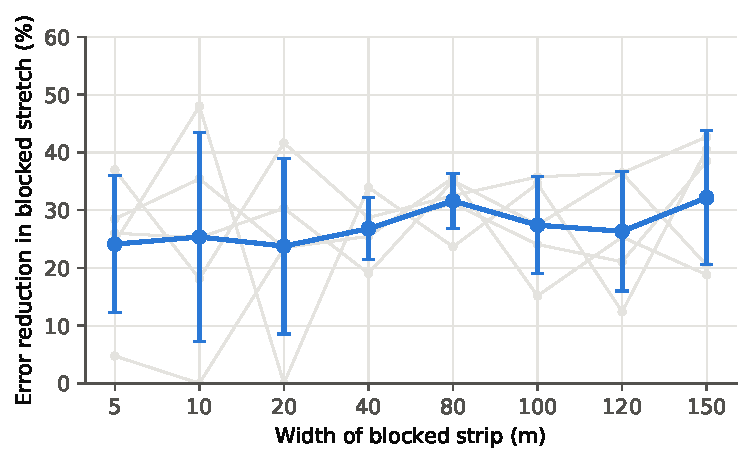
\includegraphics[width=0.7\textwidth]{fig_blocked_by_width}
  \caption{Reduction in mean error from adding history~($h=0$ to $h=5$) inside the blocked stretch, by width of the blocked strip, XGBoost. Gray lines are the five individual seeds; the blue line is their mean with $\pm1$ standard deviation.}
  \label{fig:blocked}
\end{figure}
% src: figure_scripts/make_figures_diagnostic.py blocked_by_width()
